%% -*- mode: latex -*-
%% -*- mode: latex; -*-
%% \documentclass[conference]{IEEEtran}
\documentclass{article}

\input{header-common}

%% \include{pgfplots}

\usepackage[normalem]{ulem}

% I'm not terrifically happy with the available TODO packages...
% Alternatives are `todonotes` and `todo`
%% \usepackage{todonotes}
%% \presetkeys{todonotes}{inline}{}
%% \usepackage{siunitx}
%% \usepackage{todo}


\usepackage[scaled]{helvet}
\renewcommand\familydefault{\sfdefault}
\usepackage[top=0.5in,bottom=0.5in,outer=0.5in,inner=0.5in,landscape]{geometry}
\usepackage{multicol}
%% \usepackage[pages=some]{background}
%% \backgroundsetup{
%%   scale=0.5,
%%   %% color=black,
%%   %% opacity=0.5,
%%   angle=0,
%%   contents={
%%     \includegraphics[
%%       width=\pagewidth,
%%       height=\pageheight
%%     ]
%%                     {src/figures/map.eps}
%%   }
%% }

\pagestyle{empty}

\begin{document}
%% \begin{multicols}{2}
\twocolumn

\section*{SAGE Ski Trip 2015}
Hi!
We're glad you decided to come along for the 2015 SAGE Ski Trip to \textbf{Stowe Mountain Resort} from January 23--25.
We're staying at the \textbf{Commodore's Inn}, located at \emph{823 South Main Street, Stowe, VT 05672}.
Your primary point of contacts are \textbf{Zack Webster} \emph{(\missingdata)} and \textbf{Schuyler Eldridge} \emph{(\missingdata)}.

Our itinerary is as shown in Table \ref{tab-itinerary}.
Buses will leave Boston from the George Sherman Union (775 Commonwealth Ave) at 1715.
On our way to Stowe, we'll stop for fast food in West Lebanon, NH.
On both Saturday and Sunday, the buses will leave at 0830 for Stowe Mountain Resort.
If you'd like to leave earlier or later, there is a free shuttle bus that stops at the Commodore's Inn every 30 minutes beginning at 0640.
After the bus drops us off in the Mansfield Parking Lot, you'll have immediate access to skiing on Mount Mansfield.
For rentals, lessons, and easier skiing you can head to Spruce Peak using the \emph{Over Easy Transfer Gondola}.
Lessons begin at 1000 and 1330.
The buses will pick us up from the resort at 1645 each day from the Mansfield Parking Lot.
Lifts servicing advanced terrain open at 0730 and lifts serving all terrain open between 0830 and 0900. Lifts close at 1600.

Our hotel includes complimentary breakfast from 0700--1030 and a sit-down dinner from 1830--1930.
You're on your own for lunch, but the Spruce Peak lodge has an excellent cafeteria.
\emph{Look for SAGE members in the lodge at lunch.}
We'll have some apr\`es-ski festivities in the hotel bar at 1715 on Saturday leading into dinner.

As a new feature this year, we're trying to facilitate \emph{optional} ski groups if you'd like to ski with people of a similar level.
If you're a beginner (comfortable on Green Circle terrain), groups will be organized around Lower Spruce Peak.
If you're an intermediate (comfortable on Blue Square terrain), groups will be organized around the Mansfield lifts.
Advanced skiers/riders (comfortable on Single and Double Black Diamonds), will be around Mt. Mansfield.
We'll provide more information on the buses about groups.

For any questions get in touch with either Zach or Schuyler.

\begin{table}[h]
  \vspace{-0.2in}
  \def\taw{0.14}
  \small
  \centering
  \caption{Itinerary}
  \label{tab-itinerary}
  \begin{tabular}{lcl}
    \toprule
    Day & Time & Description\\
    \midrule
    \multirow{4}{*}{
      \begin{minipage}{\taw\columnwidth}
        Friday
      \end{minipage}}
    & 1645 & Board Buses at GSU\\
    & 1715 & Buses Depart\\
    & 2000 & Food Stop in West Lebanon, NH \\
    & 2130 & Arrive at Hotel \\
    \midrule \multirow{5}{*}{
      \begin{minipage}{\taw\columnwidth}
        Saturday
    \end{minipage}}
    & 0700 & Breakfast Opens\\
    & 0830 & Buses Leave for Resort \\
    & 1645 & Buses Return to Hotel \\
    & 1715--1830 & Apr\`es-Ski in Hotel Bar\\
    & 1830--1930 & Dinner at Hotel \\
    \midrule \multirow{3}{*}{
      \begin{minipage}{\taw\columnwidth}
        Sunday
    \end{minipage}}
    & 0700 & Breakfast Opens\\
    & 0800 & Load Buses\\
    & 0830 & Buses Leave for Resort \\
    & 1645 & Buses Depart for Boston \\
    \bottomrule
  \end{tabular}
\end{table}

\begin{figure}
  \centering
  \begin{tikzpicture}
    % draw image
    \node[inner sep=0] at (current page.center)
         {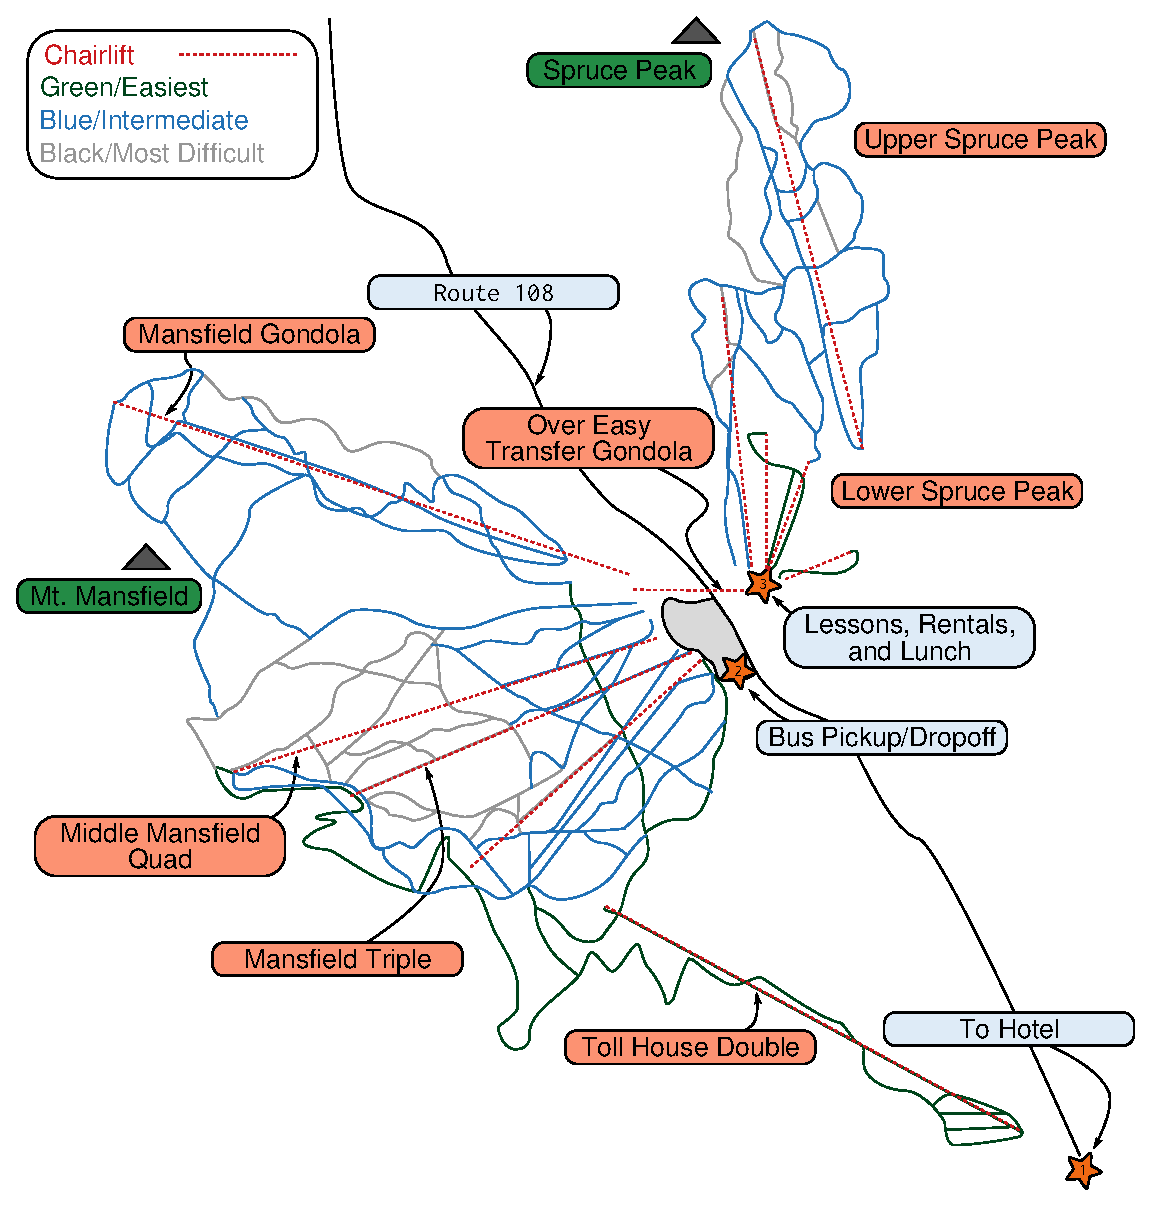
\includegraphics[width=0.9\columnwidth]{src/figures/map.eps}};
  \end{tikzpicture}
  \caption{Stowe Mountain Resort comprises two mountains, Mount Mansfield (serviced, primarily, by the \emph{Toll House Double}, \emph{Mansfield Triple}, \emph{Middle Mansfield Quad}, and \emph{Mansfield Gondola}) to the West and Spruce Peak (divided into Lower and Upper Spruce Peak) to the East.
    The \emph{Toll House Double} and \emph{Lower Spruce Peak} provide access to the easiest terrain, while all other areas and lifts have primarily intermediate and expert skiing.
    Mount Mansfield and Spruce Peak are divided by Route 108.
    You can move between them by using the \emph{Over Easy Transfer Gondola}.
    Lessons, rentals, and the main dining area are located at \emph{Lower Spruce Peak}, (3) on the map.
    Our hotel, the Commodore's Inn is located on Route 108, to the South, in the general direction of (1).
    In the morning and evening, our buses will drop off and pick up in the Mansfield parking lot at location (2).
  }
\end{figure}

%% \end{multicols}

\end{document}
